\chapter{Backend}
% This File is used to describe the different parts of the backend. That means it will include the database, the middleware, and c#/oop.
\section{Database}
\subsection{Relational Databases}
    Relational databases are a combination of two or more tables.
    These kinds of databases are so important because they are fast and very reliable. 
    The reason they are called relational is because of their table structure, that means that each table consists of many different rows and columns.
    %To be seen as a valid table input each cell in a row has to be valid.
\subsubsection{The ACID Theorem}
The Acronym ACID describes the basic guideline each database should follow. It states the four most basics points they have to fulfill to work fluently.
\begin{itemize}
    \item Atomicity: Atomicity means that changes to the data are always performed as one operation. That means that they are "all or nothing". Either all changes are applied or no changes are applied.
    \item Consistency: Consistency means that there a no problems with each transaction. That means that you each transaction have to stay in the boundaries of the previously established rules of the respective database.
    \item Isolation: Isolation means that the state of each transaction can not be seen by other transactions. That means that transactions that are started simultaneously appear as if they were launched one after the other.
    \item Durability: Durability means that transactions can not be reverted. After a transaction is done it will stay in database and can only be changed but can never be removed.
\end{itemize}
\subsubsection{The CAP Theorem}
The Acronym CAP describes three main poles 
\begin{itemize}
    \item Durability: Durability means that transactions can not be reverted. After a transaction is done it will stay in database and can only be changed but can never be removed.
\end{itemize}
\begin{figure}[h]
    \centering
    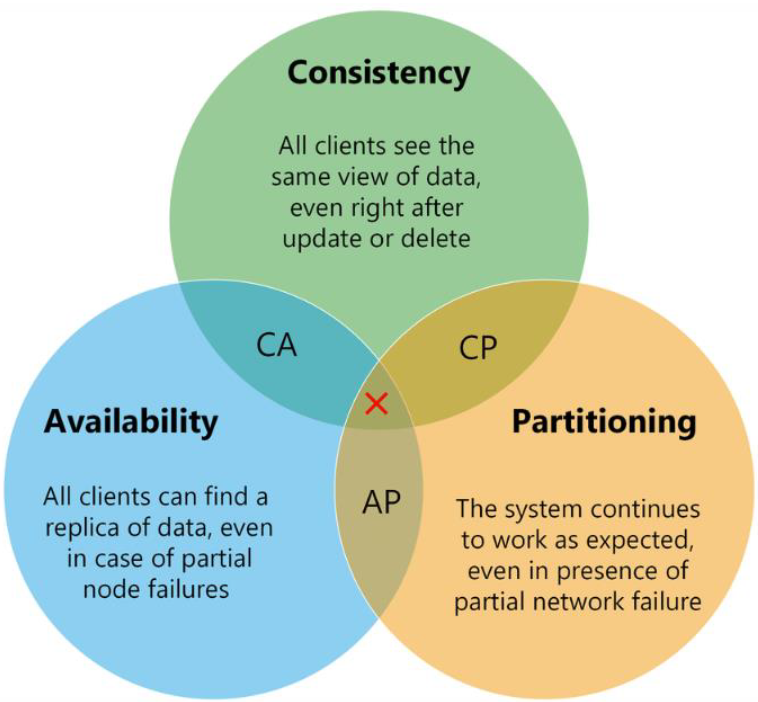
\includegraphics[width=0.4\linewidth]{images/CAP_Theorem.png}
    \caption{Venn Diagram to depict the CAP Theorem}
    \label{fig:FirstIteration-general}
    \end{figure}